{}\documentclass[letterpaper,
compress,
xcolor=x11names,
%draft,
]{beamer}
% Package imports
\usepackage{mathtools} % imports `amsmath'
\DeclareMathOperator{\sech}{sech}
\usepackage{amssymb}
\usepackage{fixltx2e}
\usepackage{lmodern}
\usepackage{movie15}
%\usepackage{media9}
\usepackage{microtype}
\usepackage{animate}
\usepackage{subcaption}
\captionsetup{compatibility=false}

% I just did this
\usepackage[english]{babel}
\usepackage[utf8]{inputenc}
\usepackage{amsmath}
\usepackage{graphicx}
\usepackage[colorinlistoftodos]{todonotes}
\usepackage{tikz}
\usetikzlibrary{tikzmark}
\usepackage{array}
\usepackage{layout}
\usepackage{multicol}
\usepackage{multirow}
\usepackage{booktabs}
%I just did this

% `beamer' configuration
\usefonttheme{professionalfonts}
\useoutertheme[subsection=false,]{miniframes}
\setbeamercolor*{alerted text}{fg=red}
\setbeamercolor*{example text}{fg=black}
\definecolor{CSU_green}{RGB}{30, 70, 43}
\definecolor{CSU_gold}{RGB}{200, 195, 114}
\setbeamercolor*{lower separation line head}{bg=CSU_gold}
\setbeamercolor*{section in head/foot}{fg=white,bg=CSU_green}
\setbeamercolor*{subsection in head/foot}{bg=white}
\setbeamercolor*{upper separation line head}{bg=CSU_gold}
\setbeamercolor*{page number in head/foot}{fg=CSU_green}
\setbeamercolor*{normal text}{fg=black,bg=white}
\setbeamercolor*{palette tertiary}{fg=black,bg=black!10}
\setbeamercolor*{palette quaternary}{fg=black,bg=black!10}
\setbeamercolor*{structure}{fg=black}
\setbeamerfont{frametitle}{shape=\scshape}
\setbeamerfont{institute}{shape=\scshape}
\setbeamerfont{section in head/foot}{shape=\scshape}
\setbeamerfont{subsection in head/foot}{shape=\scshape}
\setbeamertemplate{bibliography item}{}
\setbeamertemplate{itemize items}[ball]
\setbeamertemplate{navigation symbols}{}
\setbeamertemplate{footline}[frame number]
\usetikzlibrary{calc,arrows}
\graphicspath{{graphics/}{graphics/movies/}{graphics/images/}}
\usepackage{remreset}                  % hack to display beamer navigation
\makeatletter                          % circles even if not declaring
\@removefromreset{subsection}{section} % subsections
\makeatother                           % see: http://tex.stackexchange.com/a/2078
\setcounter{subsection}{1}             % see: https://bitbucket.org/rivanvx/beamer/issue/218

% `biblatex' configuration
\usepackage[backend=biber,
style=authortitle-comp,
]{biblatex}
\addbibresource{presentation.bib}

% `enumitem' configuration
\usepackage{enumitem}
\setlist[itemize,1]{label=\usebeamertemplate{itemize item}}
\setlist[itemize,2]{label=\usebeamertemplate{itemize subitem}}
\setlist[itemize,3]{label=\usebeamertemplate{itemize subsubitem}}
\DeclareMathOperator{\sinc}{sinc}


% `graphicx' configuration
\usepackage{graphicx}
\begin{document}
	\title{General Coding Concepts}
	%\subtitle{MATH-151:  Mathematical Algorithms in Matlab}
	\author{MATH-151:  Mathematical Algorithms in Matlab}
	\date[202X]{August 23, 2023}
	\titlegraphic{
\includegraphics[height = 3cm]{CSU_Ram_Logo.jpg}}



%%%%%%%%%%%%%%%%%%%%%%%%%%%%%%%%%%%%%%%%%%%%%%%%%%%%%%

\begin{frame}
\titlepage
\end{frame}
%%%%%%%%%%%%%%%%%%%%%%%%%%%%%%%%%%%%%%%%%%%%%%%%%%%%%%%%%
\section{Coding Concepts}

\begin{frame}{Statements and Commands}
	\footnotesize
	\begin{itemize}
		\item We communicate with the computer using a series of \textbf{statements} or \textbf{commands} that instruct the computer what to do
		\begin{itemize}
			\item It will do \textit{exactly} and \textit{only} what you command it to do 
		\end{itemize}
	\end{itemize}
	\vspace{0.5cm}
	\underline{Some examples of commands we'll make use of}
	\begin{columns}
		\begin{column}{0.45\linewidth}
			\begin{itemize}
				\item Arithmetic operators
				\begin{itemize}
					\item \texttt{6 + 3}
					\item \texttt{48 - 13}
					\item \texttt{6*17}
					\item \texttt{4096/4}
					\item \texttt{12\^{}2}
				\end{itemize}
				\item Control statements
				\begin{itemize}
					\item \texttt{if ... else ...}
					\item \texttt{for ...}
					\item \texttt{while ...}
				\end{itemize}
				
			\end{itemize}
		\end{column}
		\begin{column}{0.45\linewidth}
			\begin{itemize}
				\item Mathematical functions 
				\begin{itemize}
					\item \texttt{sin(pi)}
					\item \texttt{cos(pi/4)}
					\item \texttt{exp(2)}
					\item \texttt{log(1)}
					\item \texttt{sqrt(120)}
				\end{itemize}
				\item Presentation statements 
				\begin{itemize}
					\item \texttt{display(18/3 + 7)}
					\item \texttt{plot(x,y)}
				\end{itemize}
			\end{itemize}
		\end{column}
	\end{columns}
\end{frame}
%%%%%%%%%%%%%%%%%%%%%%%%%%%%%%%%%%%%%%%%%%%%%%%%%%%%%%%%%%
\begin{frame}{Variables and Assignment}
	\footnotesize
	\begin{itemize}
		\item Commands are great, but they aren't very useful as displayed on the previous slide. The real power of computers is the ability to keep track of many values as we perform many operations!
		\item To do this, instead of using numbers directly, we often will apply those values to variables. For example
		\begin{columns}
			\begin{column}{0.05\linewidth}
			\end{column}
			\begin{column}{0.65\linewidth}
				\scriptsize
				\begin{itemize}
					\item \texttt{x = 7;} tells the computer that wherever it sees \texttt{x} to use \texttt{7} instead.
					\item Similarly we can set \texttt{y = 10;} and see how they interact!
				\end{itemize}
			\end{column}
			\begin{column}{0.3\linewidth}
				\begin{center}
					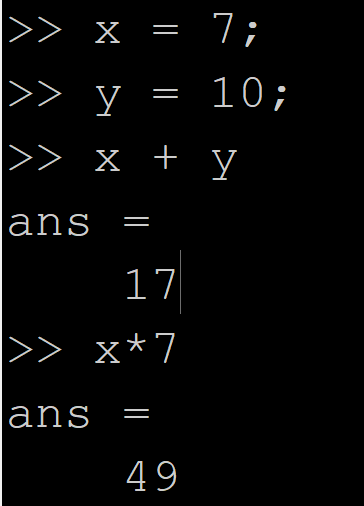
\includegraphics[height = 2cm]{Variables.png}
				\end{center}
			\end{column}
		\end{columns}
		\item This is called assigning a value to a variable. A very important use is that we can use those variables throughout our code, and even use it to update the variable itself!
		\begin{columns}
			\begin{column}{0.05\linewidth}
			\end{column}
			\begin{column}{0.65\linewidth}
				\scriptsize
				\begin{itemize}
					\item For example \texttt{x = x + 2;} is interpreted as ``take \texttt{x}, add 2 to it, and that is our new \texttt{x}"
					\item In Matlab \texttt{=} is used for assignment, so its a little different than the = you've seen in the past. Some languages use \texttt{<-} for assignment to make this more clear.
				\end{itemize}
			\end{column}
			\begin{column}{0.3\linewidth}
				\begin{center}
					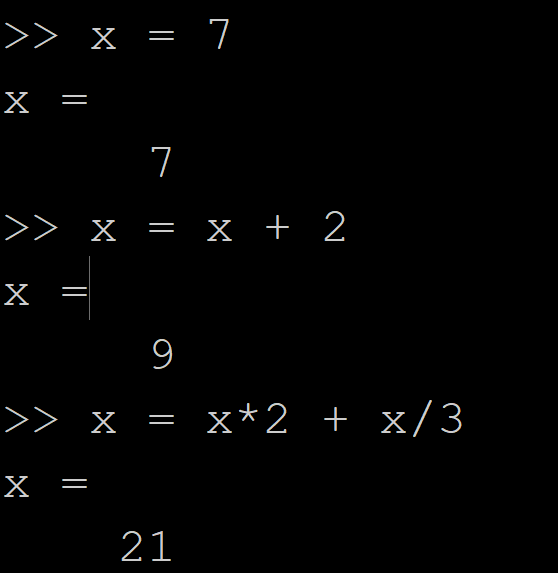
\includegraphics[height = 2cm]{VariableUpdates.png}
				\end{center}
			\end{column}
		\end{columns}
	\end{itemize}
\end{frame}
%%%%%%%%%%%%%%%%%%%%%%%%%%%%%%%%%%%%%%%%%%%%%%%%%%%%%%%%%%
\begin{frame}{The End [of a Statement]}
	\footnotesize
	\begin{columns}
		\begin{column}{0.65\linewidth}
			\begin{itemize}
				\item There are two ways to indicate to Matlab that a statement is complete.
				\begin{itemize}
					\item End of the line
						\begin{itemize}
							\item Press the enter key! Matlab will see an invisible character called the "Line Feed" and know the statement is complete
							\item Matlab will perform this statement \textbf{and print the result to the Command Window}
						\end{itemize}
					\item Semicolon (;)
						\begin{itemize}
							\item A Semicolon indicates to Matlab that a command is finished and \textbf{do not print result to Command Window} 
							\item Eventually, most of your commands will end with a semicolon.
						\end{itemize}
				\end{itemize}
			\end{itemize}
		\end{column}
		\begin{column}{0.3\linewidth}
			\begin{center}
				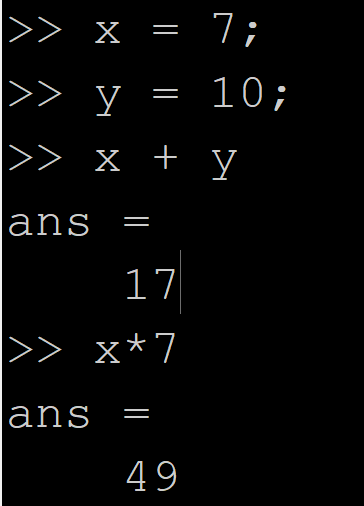
\includegraphics[height = 4cm]{Variables.png}
			\end{center}
		\end{column}
	\end{columns}
\end{frame}
%%%%%%%%%%%%%%%%%%%%%%%%%%%%%%%%%%%%%%%%%%%%%%%%%%%%%%%%%%
\begin{frame}{Comments}
	\footnotesize
	\begin{itemize}
		\item When writing code, it is always important to remember that you will have to pass it along to someone else at some point. So it is good to make sure your code is easy to read and understand
		\begin{itemize}
			\item You'll probably find that ``other person" is yourself at a later date!
		\end{itemize}
		\item Comments are lines in code that are ignored by the computer, but allow us to describe in words what we intend for the code to do
		\item In Matlab, we use the symbol \% to tell the computer that everything afterwards on that line is a comment
		\item Some helpful guidelines on effective commenting
		\begin{itemize}
			\item Describe what variables represent (also use descriptive variable names as your codes become more complicated)
			\item Focus on \textbf{what} code is doing, rather than \textbf{how} it is doing it
		\end{itemize}
	\end{itemize}
\end{frame}

%%%%%%%%%%%%%%%%%%%%%%%%%%%%%%%%%%%%%%%%%%%%%%%%%%%%%%%%%
\begin{frame}{Confusers}
	\footnotesize
	\begin{itemize}
		\item Here's two quotes I keep in mind when computing
		\begin{itemize}
			\item ``I call this a confuser, because it confuses you into thinking it has the right answer"
			\item ``All models are wrong, but some are useful"
		\end{itemize}
		\item Let's suppose I ask Matlab to compute $\sqrt{2}\sqrt{2}-2$. How about $\sin(\pi)$?
		\begin{center}
			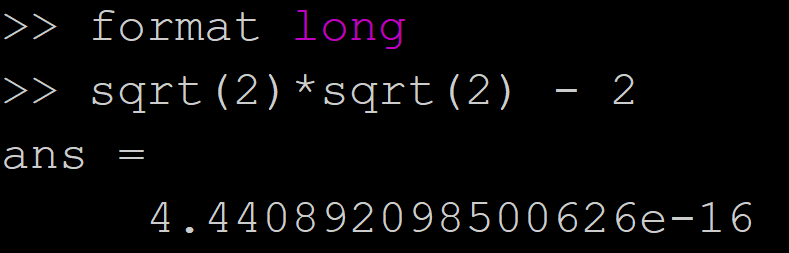
\includegraphics[height = 1cm]{sqrt2squared.png} \hspace{1cm}
			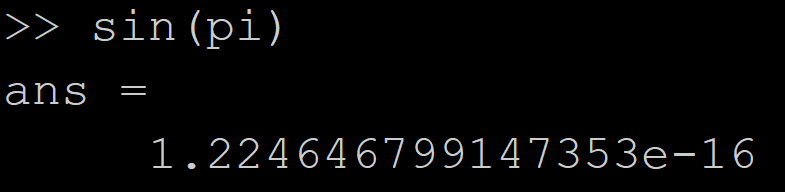
\includegraphics[height = 1cm]{sinpi.png}
		\end{center}
		\item Computers can only store a finite number of digits, so irrational numbers like $\pi$ and $\sqrt{2}$ will always be just a *little* wrong. Also, most functions (like the $\sin(x)$) are represented by a finite number of terms in their Taylor Series expansions.
		\item Computer models are still very practical and useful, just keep in mind that there is always error!
	\end{itemize}
\end{frame}

%%%%%%%%%%%%%%%%%%%%%%%%%%%%%%%%%%%%%%%%%%%%%%%%%%%%%%%%%
\section{Matlab Usage}

\begin{frame}{Installing Matlab}
	\footnotesize
	\begin{itemize}
		\item In that class we will be focusing on Matlab as our coding language \\
		\begin{center}		
			\textcolor{blue}{\href{https://www.mathworks.com/academia/tah-portal/colorado-state-university-40638290.html}{Here's the Matlab install link again!}}
			
\includegraphics[height = 3cm]{MatlabInstallSite.png}
		\end{center}
		\item The install process asks which toolboxes you want to install. This class will not require any of them, but here are some that I've used the most
		\begin{itemize}
			\item Image Processing Toolbox
			\item Navigation Toolbox
			\item Parallel Computing Toolbox
			\item Signal Processing Toolbox
			\item Statistics and Machine Learning Toolbox
		\end{itemize}
		\item Installation can take a while! It took me about an hour!
	\end{itemize}
\end{frame}
%%%%%%%%%%%%%%%%%%%%%%%%%%%%%%%%%%%%%%%%%%%%%%%%%%%%%%%%%
\begin{frame}{Matlab Demo}
	I am going to show you a quick script in Matlab to help show you around the program.
\end{frame}
%%%%%%%%%%%%%%%%%%%%%%%%%%%%%%%%%%%%%%%%%%%%%%%%%%%%%%%%%
\begin{frame}{Scripts}
	\footnotesize
	\begin{columns}
		\begin{column}{0.5\linewidth}
			\begin{itemize}
				\item One of the primary ways we will interact with Matlab is through \textbf{scripts}
				\begin{itemize}
					\scriptsize
					\item Click the "New Script" button on the command window to create a new script
				\end{itemize}
				\item These are files, \{Filename\}.m, that contain a collection of statements for Matlab, so you don't need to enter them one by one into the Command Window
				\item When you want to \textbf{execute} a script, there is a run button toward the top of the Editor window.
				\begin{itemize}
					\scriptsize
					\item You can also press F5 on your keyboard
				\end{itemize}
			\end{itemize}
		\end{column}
		\begin{column}{0.5\linewidth}
			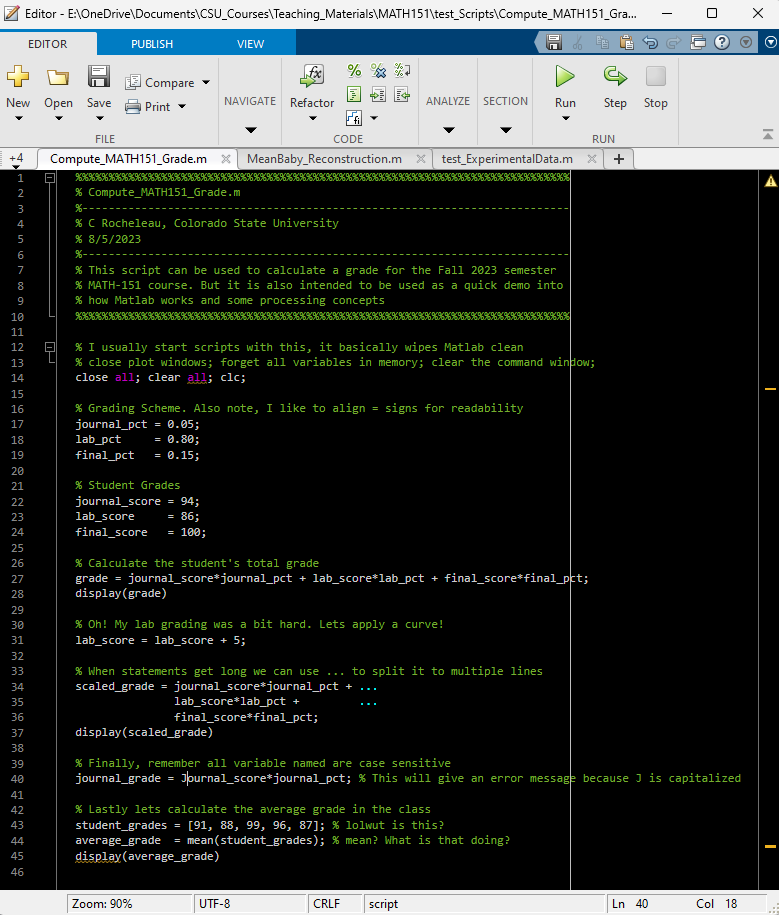
\includegraphics[width = \linewidth]{Script_example.png}
		\end{column}
	\end{columns}
\end{frame}
%%%%%%%%%%%%%%%%%%%%%%%%%%%%%%%%%%%%%%%%%%%%%%%%%%%%%%%%%
\begin{frame}{Errors}
	\footnotesize
	\begin{itemize}
		\item An error occurs when Matlab tries to process a statement, but cannot interpret it
		\item It will respond by beeping angrily and posting an \textbf{error message} to the command window. Telling you where the error occurred, and what's wrong
		\begin{center}
		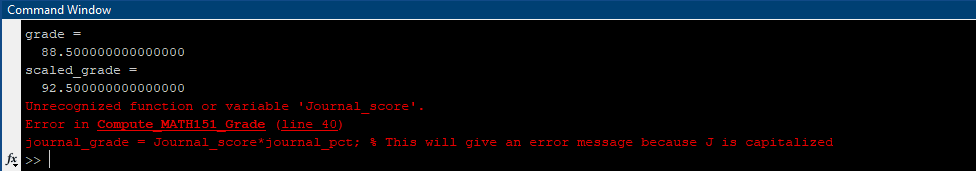
\includegraphics[width = \linewidth]{error_message.png}
		\end{center}
		\item In this case it is trying to use \texttt{Journal\_score}, but the variable doesn't exist.
		\item The variable \texttt{journal\_score}, does exist though! Variable names are case-sensitive
		\item A lot of your time coding will be fixing errors. Don't get discouraged by them, they are a learning opportunity!
		\begin{itemize}
			\item A lot of time they are typos though...
		\end{itemize}
	\end{itemize}
\end{frame}

%%%%%%%%%%%%%%%%%%%%%%%%%%%%%%%%%%%%%%%%%%%%%%%%%%%%%%%%%
\end{document}